\section{Trabajo de la fuerza eléctrica}

Cuando una carga eléctrica se encuentra en un campo eléctrico, experimenta una
fuerza. Si la carga se desplaza, esa fuerza puede realizar trabajo.

El concepto de trabajo permite estudiar muchas interacciones eléctricas sin tener
que analizar directamente el movimiento mediante fuerzas y aceleraciones en cada
instante.

Para un desplazamiento infinitesimal, el trabajo realizado por la fuerza eléctrica es

\[
dW_e=\vec F_e\cdot d\vec r.
\]

Por tanto, cuando una carga se mueve desde un punto \(A\) hasta un punto \(B\),

\begin{equation}
\boxed{
W_{e,A\to B}
=
\int_A^B \vec F_e\cdot d\vec r
}.
\label{eq:trabajo_fuerza_electrica}
\end{equation}

En términos de componentes rectangulares,

\begin{equation}
\boxed{
W_{e,A\to B}
=
\int_A^B
\left(
F_x\,dx+F_y\,dy+F_z\,dz
\right)
}.
\label{eq:trabajo_electrico_componentes}
\end{equation}

Como

\[
F_x=qE_x,\qquad
F_y=qE_y,\qquad
F_z=qE_z,
\]

también puede escribirse

\begin{equation}
\boxed{
W_{e,A\to B}
=
q\int_A^B
\left(
E_x\,dx+E_y\,dy+E_z\,dz
\right)
}.
\label{eq:trabajo_campo_componentes}
\end{equation}

\begin{idea}

El trabajo depende únicamente de la componente de la fuerza que actúa en la
dirección del desplazamiento.

Una componente perpendicular al desplazamiento no realiza trabajo.

\end{idea}


\section{La fuerza electrostática es conservativa}

Una característica fundamental de la fuerza electrostática es que se trata de una
\textbf{fuerza conservativa}.

Esto significa que el trabajo realizado por la fuerza eléctrica al mover una carga
entre dos puntos depende únicamente de las posiciones inicial y final.

No depende de la trayectoria seguida entre ellas.

Si una carga puede desplazarse desde \(A\) hasta \(B\) siguiendo dos trayectorias
diferentes,

\[
W_{e,A\to B}^{(1)}
=
W_{e,A\to B}^{(2)}.
\]

Por tanto,

\[
\boxed{
W_{e,A\to B}
\text{ es independiente de la trayectoria}
}.
\]


\subsection{Trabajo en una trayectoria cerrada}

Si la carga realiza un recorrido cerrado y regresa al punto inicial, las posiciones
inicial y final coinciden.

Por ello,

\begin{equation}
\boxed{
\oint \vec F_e\cdot d\vec r=0
}.
\label{eq:trabajo_cerrado_electrico}
\end{equation}

Esta propiedad permite definir una energía potencial asociada con la interacción
eléctrica.


\section{Energía potencial eléctrica}

Como la fuerza electrostática es conservativa, podemos asociar a la configuración
de las cargas una magnitud llamada \textbf{energía potencial eléctrica}.

\begin{definicion}[Energía potencial eléctrica]

La energía potencial eléctrica \(U\) es una magnitud escalar asociada con la
configuración de un sistema de cargas eléctricas.

Su cambio está relacionado con el trabajo realizado por la fuerza eléctrica.

\end{definicion}

Si una carga se desplaza desde \(A\) hasta \(B\),

\begin{equation}
\boxed{
\Delta U=U_B-U_A=-W_{e,A\to B}
}.
\label{eq:cambio_energia_potencial}
\end{equation}

Equivalentemente,

\begin{equation}
\boxed{
W_{e,A\to B}=U_A-U_B
}.
\label{eq:trabajo_cambio_energia}
\end{equation}

Por tanto,

\[
W_e>0
\Longrightarrow
\Delta U<0,
\]

mientras que

\[
W_e<0
\Longrightarrow
\Delta U>0.
\]

\begin{idea}

Cuando la fuerza eléctrica realiza trabajo positivo, la energía potencial eléctrica
del sistema disminuye.

Cuando la fuerza eléctrica realiza trabajo negativo, la energía potencial aumenta.

\end{idea}


\subsection{La energía potencial pertenece al sistema}

Es importante interpretar correctamente \(U\).

Una carga aislada no posee por sí sola una energía potencial eléctrica determinada.

La energía potencial eléctrica corresponde a la \textbf{configuración del sistema de
cargas}.

Por ejemplo, para dos cargas puntuales, \(U\) depende de

\begin{itemize}
    \item el valor de ambas cargas;
    \item sus signos;
    \item la distancia que las separa.
\end{itemize}

Por ello, al modificar la separación entre las cargas cambia la energía potencial
del sistema.


\subsection{Unidad de la energía potencial eléctrica}

En el Sistema Internacional,

\[
\boxed{[U]=\si{\joule}}.
\]

La energía potencial eléctrica, al igual que cualquier energía, es una magnitud
escalar.


\section{Trabajo externo y energía potencial}

Supongamos que una fuerza externa desplaza lentamente una carga desde \(A\) hasta
\(B\), de manera que su energía cinética no cambie apreciablemente.

En ese caso, la fuerza externa debe compensar a la fuerza eléctrica.

El trabajo realizado por la fuerza externa cumple

\begin{equation}
\boxed{
W_{\text{ext}}=\Delta U
}
\label{eq:trabajo_externo_deltaU}
\end{equation}

si el proceso se realiza lentamente y no intervienen otros mecanismos de intercambio
de energía.

Al mismo tiempo,

\[
W_e=-\Delta U.
\]

Por tanto,

\[
\boxed{
W_{\text{ext}}=-W_e
}.
\]

\begin{idea}

Existen dos formas equivalentes de interpretar un aumento de energía potencial:

\begin{itemize}
    \item el campo eléctrico realiza trabajo negativo;
    \item un agente externo debe realizar trabajo positivo contra la fuerza eléctrica.
\end{itemize}

\end{idea}


\section{Cambio de energía potencial en un campo eléctrico}

Como

\[
W_e
=
q\int_A^B
\left(
E_x\,dx+E_y\,dy+E_z\,dz
\right),
\]

y

\[
\Delta U=-W_e,
\]

resulta

\begin{equation}
\boxed{
\Delta U
=
-q\int_A^B
\left(
E_x\,dx+E_y\,dy+E_z\,dz
\right)
}.
\label{eq:deltaU_campo_componentes}
\end{equation}

Esta expresión permite calcular cambios de energía potencial cuando se conoce el campo
eléctrico.


\subsection{Campo eléctrico uniforme}

Si el campo es uniforme, sus componentes son constantes y pueden salir de la integral:

\[
\Delta U
=
-q
\left(
E_x\Delta x+
E_y\Delta y+
E_z\Delta z
\right).
\]

Por tanto,

\begin{equation}
\boxed{
\Delta U
=
-q
\left(
E_x\Delta x+
E_y\Delta y+
E_z\Delta z
\right)
}.
\label{eq:deltaU_campo_uniforme}
\end{equation}

En una dimensión, si el campo está dirigido sobre el eje \(x\),

\begin{equation}
\boxed{
\Delta U=-qE_x\Delta x
}.
\label{eq:deltaU_uniforme_1d}
\end{equation}


\subsection{Ejemplo: trabajo y energía en un campo uniforme}

\begin{ejemplo}

Una carga

\[
q=+\SI{3.0}{\micro\coulomb}
\]

se desplaza en un campo eléctrico uniforme cuyas componentes son

\[
E_x=\SI{200}{\newton\per\coulomb},
\qquad
E_y=-\SI{100}{\newton\per\coulomb}.
\]

Durante el desplazamiento,

\[
\Delta x=\SI{0.40}{\metre},
\qquad
\Delta y=\SI{0.20}{\metre}.
\]

Determine el trabajo realizado por la fuerza eléctrica y el cambio de energía
potencial.

\end{ejemplo}

Como el campo es uniforme,

\[
W_e=q(E_x\Delta x+E_y\Delta y).
\]

Sustituyendo,

\[
W_e
=
(3.0\times10^{-6})
\left[
(200)(0.40)+(-100)(0.20)
\right].
\]

Entonces,

\[
W_e
=
(3.0\times10^{-6})(80-20).
\]

Por tanto,

\[
\boxed{W_e=\SI{1.8e-4}{\joule}}.
\]

El cambio de energía potencial es

\[
\Delta U=-W_e,
\]

de modo que

\[
\boxed{\Delta U=-\SI{1.8e-4}{\joule}}.
\]

La fuerza eléctrica realiza trabajo positivo y, en consecuencia, la energía potencial
del sistema disminuye.


\section{Elección del cero de energía potencial}

El valor absoluto de la energía potencial depende del nivel de referencia elegido.

Lo físicamente significativo es el cambio

\[
\Delta U=U_B-U_A.
\]

Podemos sumar una constante a todos los valores de \(U\) sin modificar ninguna
predicción física.

Para sistemas de cargas puntuales aisladas se adopta normalmente la referencia

\begin{equation}
\boxed{
U=0
\qquad\text{cuando}\qquad
r\to\infty
}.
\label{eq:cero_energia_infinito}
\end{equation}

Esta elección significa que consideramos nula la energía de interacción cuando las
cargas están infinitamente separadas.


\section{Energía potencial eléctrica de dos cargas puntuales}

Consideremos dos cargas puntuales \(q_1\) y \(q_2\) separadas una distancia \(r\).

Tomando

\[
U(\infty)=0,
\]

la energía potencial eléctrica del sistema es

\begin{equation}
\boxed{
U=k\frac{q_1q_2}{r}
}.
\label{eq:energia_potencial_dos_cargas}
\end{equation}

donde

\[
k=\frac{1}{4\pi\varepsilon_0}.
\]

\begin{advertencia}

En esta expresión \textbf{no se utiliza valor absoluto} en el producto de las cargas.

\[
U=k\frac{q_1q_2}{r}.
\]

El signo de \(q_1q_2\) determina el signo de la energía potencial.

\end{advertencia}


\section{Significado del signo de la energía potencial}

\subsection{Cargas del mismo signo}

Si las cargas tienen el mismo signo,

\[
q_1q_2>0.
\]

Entonces,

\[
\boxed{U>0}.
\]

Para acercar lentamente dos cargas que se repelen desde una separación infinita hasta
una distancia finita, un agente externo debe realizar trabajo positivo.

La energía aportada queda almacenada como energía potencial eléctrica del sistema.


\subsection{Cargas de signos opuestos}

Si las cargas tienen signos opuestos,

\[
q_1q_2<0.
\]

Entonces,

\[
\boxed{U<0}.
\]

Al acercarse desde el infinito, las cargas se atraen y la fuerza eléctrica realiza
trabajo positivo.

Por ello, la energía potencial del sistema disminuye por debajo del nivel elegido como
cero.

Para separar nuevamente las cargas hasta el infinito debe suministrarse energía al
sistema.


\begin{idea}

Con la referencia \(U(\infty)=0\),

\[
\boxed{
\begin{array}{c|c}
\text{Interacción} & U\\
\hline
\text{cargas del mismo signo} & U>0\\
\text{cargas de signos opuestos} & U<0
\end{array}
}
\]

\end{idea}


\section{Comportamiento de \(U\) con la distancia}

Para dos cargas puntuales,

\[
U=k\frac{q_1q_2}{r}.
\]

Por tanto,

\[
U\propto\frac{1}{r}.
\]

Si las cargas tienen el mismo signo, \(U\) es positiva y aumenta cuando las cargas
se acercan.

Si tienen signos opuestos, \(U\) es negativa y se vuelve más negativa cuando disminuye
la distancia.


\begin{center}
\begin{tikzpicture}[>=Latex,scale=0.9]

\draw[->] (0,-3.2) -- (0,3.2) node[above] {$U$};
\draw[->] (0,0) -- (6.2,0) node[right] {$r$};

\draw[thick,domain=0.55:6,samples=80]
plot (\x,{1.6/\x});

\draw[thick,domain=0.55:6,samples=80]
plot (\x,{-1.6/\x});

\node[right] at (3.8,0.6) {$q_1q_2>0$};
\node[right] at (3.8,-0.6) {$q_1q_2<0$};

\draw[dashed] (0,-0.02) -- (6,-0.02);

\end{tikzpicture}
\end{center}

En ambos casos,

\[
\boxed{U\to0\quad\text{cuando}\quad r\to\infty}.
\]


\section{Obtención de la fuerza a partir de la energía potencial}

En un movimiento radial unidimensional, la fuerza puede relacionarse con la energía
potencial mediante

\begin{equation}
\boxed{
F_r=-\frac{dU}{dr}
}.
\label{eq:fuerza_desde_energia}
\end{equation}

Para dos cargas,

\[
U=k\frac{q_1q_2}{r}.
\]

Entonces,

\[
\frac{dU}{dr}
=
-k\frac{q_1q_2}{r^2}.
\]

Por tanto,

\[
F_r
=
-\frac{dU}{dr}
=
k\frac{q_1q_2}{r^2}.
\]

El signo contiene información sobre el sentido radial de la fuerza:

\[
q_1q_2>0
\Longrightarrow
F_r>0,
\]

correspondiente a una interacción repulsiva, mientras que

\[
q_1q_2<0
\Longrightarrow
F_r<0,
\]

correspondiente a una interacción atractiva.

Así, la ley de Coulomb también puede obtenerse a partir de la función de energía
potencial.


\section{Ejemplo: energía potencial de dos cargas}

\begin{ejemplo}

Dos cargas puntuales

\[
q_1=+\SI{3.0}{\micro\coulomb},
\qquad
q_2=-\SI{2.0}{\micro\coulomb}
\]

se encuentran separadas

\[
r=\SI{0.40}{\metre}.
\]

Determine la energía potencial eléctrica del sistema.

\end{ejemplo}

Aplicamos

\[
U=k\frac{q_1q_2}{r}.
\]

Sustituyendo,

\[
U
=
(8.99\times10^9)
\frac{(3.0\times10^{-6})(-2.0\times10^{-6})}{0.40}.
\]

Entonces,

\[
\boxed{U\approx-\SI{0.135}{\joule}}.
\]

El resultado es negativo porque las cargas tienen signos opuestos.

Con la referencia \(U(\infty)=0\), sería necesario suministrar
\(\SI{0.135}{\joule}\) al sistema para separar lentamente las cargas hasta una
distancia infinita.


\section{Trabajo al cambiar la separación entre dos cargas}

Si dos cargas pasan de una separación inicial \(r_i\) a una separación final \(r_f\),

\[
U_i=k\frac{q_1q_2}{r_i},
\qquad
U_f=k\frac{q_1q_2}{r_f}.
\]

El cambio de energía potencial es

\begin{equation}
\boxed{
\Delta U
=
kq_1q_2
\left(
\frac{1}{r_f}
-
\frac{1}{r_i}
\right)
}.
\label{eq:deltaU_dos_cargas}
\end{equation}

El trabajo realizado por la fuerza eléctrica es

\begin{equation}
\boxed{
W_e
=
kq_1q_2
\left(
\frac{1}{r_i}
-
\frac{1}{r_f}
\right)
}.
\label{eq:trabajo_dos_cargas}
\end{equation}


\subsection{Trabajo para ensamblar dos cargas}

Si la configuración inicial corresponde a una separación infinita,

\[
r_i\to\infty,
\]

entonces

\[
U_i=0.
\]

Si una fuerza externa acerca lentamente las cargas hasta una distancia \(r\),

\[
W_{\text{ext}}=\Delta U.
\]

Por tanto,

\begin{equation}
\boxed{
W_{\text{ext}}
=
k\frac{q_1q_2}{r}
}.
\label{eq:trabajo_ensamblaje_dos_cargas}
\end{equation}

El trabajo del campo eléctrico es

\[
\boxed{
W_e=-k\frac{q_1q_2}{r}
}.
\]


\section{Energía potencial de un sistema de cargas puntuales}

Cuando existen más de dos cargas, la energía potencial total del sistema es la suma
de las energías de interacción de todos los pares diferentes.

Para \(N\) cargas,

\begin{equation}
\boxed{
U
=
k\sum_{i<j}
\frac{q_iq_j}{r_{ij}}
}.
\label{eq:energia_sistema_cargas}
\end{equation}

donde \(r_{ij}\) es la distancia entre las cargas \(q_i\) y \(q_j\).

La condición

\[
i<j
\]

garantiza que cada par se cuente una sola vez.


\subsection{Sistema de tres cargas}

Para tres cargas,

\begin{equation}
\boxed{
U
=
k
\left(
\frac{q_1q_2}{r_{12}}
+
\frac{q_1q_3}{r_{13}}
+
\frac{q_2q_3}{r_{23}}
\right)
}.
\label{eq:energia_tres_cargas}
\end{equation}

Existen tres pares:

\[
(1,2),\qquad(1,3),\qquad(2,3).
\]

\begin{advertencia}

No deben sumarse las fuerzas ni las magnitudes de las cargas para obtener \(U\).

La energía potencial total se obtiene sumando las energías de interacción de
\textbf{cada par}.

\end{advertencia}


\section{Interpretación como trabajo de ensamblaje}

La energía potencial de un sistema puede interpretarse como el trabajo que debe
realizar un agente externo para construir lentamente la configuración llevando las
cargas desde separaciones infinitas hasta sus posiciones finales.

Consideremos tres cargas.

La primera puede colocarse sin realizar trabajo de interacción, porque todavía no
existen otras cargas en el sistema.

Al colocar la segunda aparece la interacción entre \(q_1\) y \(q_2\).

Al colocar la tercera, ésta interactúa tanto con \(q_1\) como con \(q_2\).

El trabajo total queda

\[
U
=
U_{12}+U_{13}+U_{23}.
\]

El resultado final no depende del orden en que se ensamblen las cargas, lo cual es
otra consecuencia del carácter conservativo de la interacción electrostática.


\section{Ejemplo: sistema de tres cargas}

\begin{ejemplo}

Tres cargas puntuales se encuentran en los vértices de un triángulo rectángulo:

\[
q_1=+\SI{2.0}{\micro\coulomb},
\qquad
q_2=-\SI{3.0}{\micro\coulomb},
\qquad
q_3=+\SI{4.0}{\micro\coulomb}.
\]

Las distancias entre ellas son

\[
r_{12}=\SI{0.30}{\metre},
\qquad
r_{13}=\SI{0.40}{\metre},
\qquad
r_{23}=\SI{0.50}{\metre}.
\]

Determine la energía potencial eléctrica del sistema.

\end{ejemplo}

La geometría puede representarse como

\begin{center}
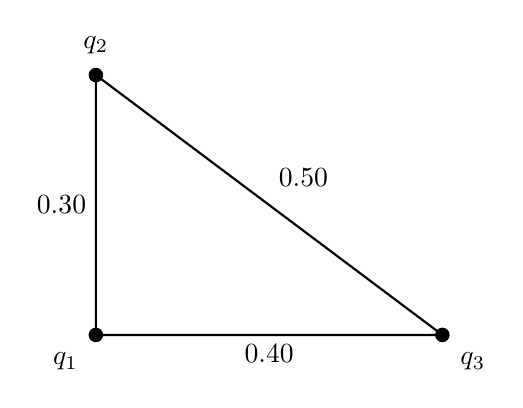
\begin{tikzpicture}[scale=1.1]

\coordinate (A) at (0,0);
\coordinate (B) at (0,3);
\coordinate (C) at (4,0);

\draw[thick] (A) -- (B) -- (C) -- cycle;

\filldraw (A) circle (2.2pt)
node[below left=3pt] {$q_1$};

\filldraw (B) circle (2.2pt)
node[above=4pt] {$q_2$};

\filldraw (C) circle (2.2pt)
node[below right=3pt] {$q_3$};

\node[left] at (0,1.5) {\(\SI{0.30}{\metre}\)};
\node[below] at (2,0) {\(\SI{0.40}{\metre}\)};
\node[above right] at (2,1.6) {\(\SI{0.50}{\metre}\)};

\end{tikzpicture}
\end{center}

Para tres cargas,

\[
U
=
k
\left(
\frac{q_1q_2}{r_{12}}
+
\frac{q_1q_3}{r_{13}}
+
\frac{q_2q_3}{r_{23}}
\right).
\]

Calculamos cada interacción:

\[
U_{12}
=
(8.99\times10^9)
\frac{(2.0\times10^{-6})(-3.0\times10^{-6})}{0.30}
\approx-\SI{0.180}{\joule},
\]

\[
U_{13}
=
(8.99\times10^9)
\frac{(2.0\times10^{-6})(4.0\times10^{-6})}{0.40}
\approx+\SI{0.180}{\joule},
\]

\[
U_{23}
=
(8.99\times10^9)
\frac{(-3.0\times10^{-6})(4.0\times10^{-6})}{0.50}
\approx-\SI{0.216}{\joule}.
\]

Sumamos las tres energías:

\[
U=U_{12}+U_{13}+U_{23}.
\]

Entonces,

\[
U=-0.180+0.180-0.216.
\]

Por tanto,

\[
\boxed{U\approx-\SI{0.216}{\joule}}.
\]

La energía total es negativa porque, para esta configuración, las interacciones
atractivas predominan energéticamente sobre la interacción repulsiva.


\section{Número de pares en un sistema}

Para \(N\) cargas puntuales, el número de pares diferentes es

\begin{equation}
\boxed{
N_{\text{pares}}
=
\frac{N(N-1)}{2}
}.
\label{eq:numero_pares}
\end{equation}

Por ejemplo,

\[
N=2\Longrightarrow1\text{ par},
\]

\[
N=3\Longrightarrow3\text{ pares},
\]

\[
N=4\Longrightarrow6\text{ pares}.
\]

Esta relación resulta útil para comprobar que ninguna interacción se haya omitido o
contado dos veces.


\section{Energía potencial y conservación de la energía}

Cuando sobre un sistema sólo actúan fuerzas electrostáticas conservativas, la suma de
la energía cinética \(K\) y la energía potencial eléctrica \(U\) permanece constante.

\begin{equation}
\boxed{
K_i+U_i=K_f+U_f
}.
\label{eq:conservacion_energia_electrica}
\end{equation}

Equivalentemente,

\[
\boxed{
\Delta K+\Delta U=0
}.
\]

Como

\[
\Delta U=-W_e
\]

y, por el teorema trabajo--energía,

\[
\Delta K=W_e,
\]

obtenemos nuevamente

\[
\Delta K=-\Delta U.
\]


\subsection{Interpretación}

Si

\[
U_f<U_i,
\]

entonces

\[
K_f>K_i.
\]

La energía potencial perdida se transforma en energía cinética.

Si

\[
U_f>U_i,
\]

entonces

\[
K_f<K_i.
\]

Parte de la energía cinética se transforma en energía potencial.


\section{Partícula liberada desde el reposo}

Si una partícula se libera desde el reposo,

\[
K_i=0.
\]

La conservación de la energía queda

\[
U_i=K_f+U_f.
\]

Por tanto,

\[
K_f=U_i-U_f.
\]

Como

\[
K_f=\frac12mv_f^2,
\]

se obtiene

\begin{equation}
\boxed{
\frac12mv_f^2=U_i-U_f
}.
\label{eq:velocidad_desde_energia_electrica}
\end{equation}

Así,

\begin{equation}
\boxed{
v_f=
\sqrt{\frac{2(U_i-U_f)}{m}}
}
\label{eq:velocidad_final_electrica}
\end{equation}

si el valor dentro de la raíz es físicamente permitido.


\section{Ejemplo: conversión de energía potencial en cinética}

\begin{ejemplo}

Una carga fija

\[
Q=+\SI{2.0}{\micro\coulomb}
\]

y una partícula de carga

\[
q=+\SI{1.0}{\micro\coulomb}
\]

y masa

\[
m=\SI{2.0e-3}{\kilogram}
\]

están inicialmente separadas

\[
r_i=\SI{0.20}{\metre}.
\]

La partícula se libera desde el reposo. Determine su rapidez cuando la separación
sea

\[
r_f=\SI{0.50}{\metre}.
\]

\end{ejemplo}

Como las dos cargas son positivas, la interacción es repulsiva. Al liberarla, la
partícula se aleja de la carga fija.

La energía potencial inicial es

\[
U_i=k\frac{Qq}{r_i}.
\]

Sustituyendo,

\[
U_i
=
(8.99\times10^9)
\frac{(2.0\times10^{-6})(1.0\times10^{-6})}{0.20}
=
\SI{8.99e-2}{\joule}.
\]

La energía potencial final es

\[
U_f
=
(8.99\times10^9)
\frac{(2.0\times10^{-6})(1.0\times10^{-6})}{0.50}
=
\SI{3.60e-2}{\joule}.
\]

Como la partícula parte del reposo,

\[
K_i=0.
\]

Aplicamos conservación de la energía:

\[
U_i=K_f+U_f.
\]

Por tanto,

\[
K_f=U_i-U_f.
\]

Entonces,

\[
K_f=0.0899-0.0360
=\SI{5.39e-2}{\joule}.
\]

Utilizamos

\[
K_f=\frac12mv_f^2.
\]

Despejando,

\[
v_f=\sqrt{\frac{2K_f}{m}}.
\]

Sustituyendo,

\[
v_f
=
\sqrt{
\frac{2(5.39\times10^{-2})}
{2.0\times10^{-3}}
}.
\]

Por tanto,

\[
\boxed{v_f\approx\SI{7.3}{\metre\per\second}}.
\]

La disminución de energía potencial eléctrica se transforma en energía cinética.


\section{Movimiento de cargas del mismo signo}

Consideremos dos cargas del mismo signo.

Su energía potencial es positiva:

\[
U=k\frac{|q_1q_2|}{r}.
\]

Si pueden moverse libremente, la fuerza repulsiva tiende a aumentar su separación.

Al aumentar \(r\),

\[
U\downarrow.
\]

Si no existen otras formas de intercambio de energía,

\[
K\uparrow.
\]

Por tanto,

\[
\boxed{
\text{repulsión espontánea}
\Longrightarrow
U\downarrow,\quad K\uparrow
}.
\]


\section{Movimiento de cargas de signos opuestos}

Para cargas de signos opuestos,

\[
U<0.
\]

Si las cargas pueden acercarse libremente, la atracción reduce la distancia.

Al disminuir \(r\), la energía potencial se hace más negativa:

\[
U\downarrow.
\]

La energía cinética aumenta:

\[
K\uparrow.
\]

Así,

\[
\boxed{
\text{atracción espontánea}
\Longrightarrow
U\downarrow,\quad K\uparrow
}.
\]

Aunque en los dos casos \(U\) disminuye durante el movimiento espontáneo, el
comportamiento de la separación es diferente:

\begin{itemize}
    \item cargas del mismo signo: se separan;
    \item cargas de signos opuestos: se acercan.
\end{itemize}


\section{Trabajo necesario para separar cargas de signos opuestos}

Supongamos que dos cargas de signos opuestos están inicialmente separadas una distancia
\(r_i\).

Su energía potencial es

\[
U_i=k\frac{q_1q_2}{r_i}<0.
\]

Si se separan lentamente hasta el infinito,

\[
U_f=0.
\]

El trabajo externo necesario es

\[
W_{\text{ext}}=U_f-U_i.
\]

Por tanto,

\begin{equation}
\boxed{
W_{\text{ext}}
=
-k\frac{q_1q_2}{r_i}
}
\label{eq:trabajo_separar_opuestas}
\end{equation}

que es positivo porque

\[
q_1q_2<0.
\]

Esto representa la energía mínima que debe suministrarse para separar lentamente el
par hasta una distancia infinita.


\section{Trabajo necesario para acercar cargas del mismo signo}

Si dos cargas del mismo signo se encuentran inicialmente en el infinito,

\[
U_i=0.
\]

Para acercarlas lentamente hasta una distancia \(r\),

\[
U_f=k\frac{q_1q_2}{r}>0.
\]

Por tanto,

\[
\boxed{
W_{\text{ext}}
=
k\frac{q_1q_2}{r}>0
}.
\]

El agente externo debe realizar trabajo positivo contra la repulsión eléctrica.


\section{Energía potencial total positiva, negativa o nula}

En un sistema de varias cargas, no basta con observar los signos individuales.

La energía total es

\[
U
=
k\sum_{i<j}
\frac{q_iq_j}{r_{ij}}.
\]

Puede ocurrir que algunas interacciones sean positivas y otras negativas.

Por ello,

\[
U>0,
\qquad
U<0
\qquad\text{o}\qquad
U=0
\]

dependiendo de los valores de las cargas y de las distancias entre ellas.

\begin{advertencia}

Que la carga neta total del sistema sea cero no implica que su energía potencial sea
cero.

La energía depende de todas las interacciones por pares y de sus separaciones.

\end{advertencia}


\section{Energía potencial y configuración}

Dos sistemas pueden contener exactamente las mismas cargas y tener energías
potenciales diferentes si las cargas están ubicadas de manera distinta.

Por tanto,

\[
\boxed{
U\text{ depende de la configuración espacial del sistema}
}.
\]

Modificar una distancia \(r_{ij}\) cambia solamente los términos de energía asociados
con las interacciones que dependen de esa distancia.


\section{Errores y confusiones frecuentes}

\begin{errorfrecuente}

\textbf{Confundir fuerza eléctrica con energía potencial eléctrica.}

La fuerza se mide en newtons y es una magnitud vectorial.

La energía potencial se mide en joules y es una magnitud escalar.

\end{errorfrecuente}


\begin{errorfrecuente}

\textbf{Pensar que una carga aislada posee por sí sola una energía potencial eléctrica.}

La energía potencial está asociada con la configuración de un sistema de cargas.

\end{errorfrecuente}


\begin{errorfrecuente}

\textbf{Usar valor absoluto en}

\[
U=k\frac{q_1q_2}{r}.
\]

Esto elimina información física esencial.

Debe conservarse el signo del producto \(q_1q_2\).

\end{errorfrecuente}


\begin{errorfrecuente}

\textbf{Pensar que \(U<0\) significa que la energía es incorrecta o imposible.}

La energía potencial puede ser negativa porque su cero es una referencia elegida.

Con \(U(\infty)=0\), un par de cargas de signos opuestos tiene energía potencial
negativa.

\end{errorfrecuente}


\begin{errorfrecuente}

\textbf{Confundir el trabajo realizado por el campo con el trabajo de una fuerza
externa.}

Para un desplazamiento cuasiestático,

\[
W_e=-\Delta U,
\]

mientras que

\[
W_{\text{ext}}=\Delta U.
\]

\end{errorfrecuente}


\begin{errorfrecuente}

\textbf{Pensar que si el campo realiza trabajo positivo la energía potencial aumenta.}

Ocurre lo contrario:

\[
W_e>0
\Longrightarrow
\Delta U<0.
\]

\end{errorfrecuente}


\begin{errorfrecuente}

\textbf{Contar dos veces una interacción en un sistema de cargas.}

Los pares

\[
(q_i,q_j)
\]

y

\[
(q_j,q_i)
\]

representan la misma interacción.

Cada par se incluye una sola vez.

\end{errorfrecuente}


\begin{errorfrecuente}

\textbf{Incluir la interacción de una carga consigo misma.}

En la expresión

\[
U=k\sum_{i<j}\frac{q_iq_j}{r_{ij}},
\]

no existe ningún término con

\[
i=j.
\]

\end{errorfrecuente}


\begin{errorfrecuente}

\textbf{Usar conservación de la energía mecánica cuando existen mecanismos externos
que realizan trabajo y omitirlos.}

La expresión

\[
K_i+U_i=K_f+U_f
\]

es válida cuando no existe transferencia adicional de energía al sistema mediante
fuerzas externas no conservativas u otros mecanismos.

\end{errorfrecuente}


\begin{errorfrecuente}

\textbf{Suponer que una energía potencial total negativa implica necesariamente una
configuración de equilibrio estable.}

El signo de \(U\) por sí solo no determina la estabilidad.

La estabilidad depende de cómo cambia la energía ante pequeñas modificaciones de la
configuración.

\end{errorfrecuente}


\section{Preguntas para comprobar comprensión}

\begin{enumerate}
    \item ¿Qué significa que la fuerza electrostática sea conservativa?

    \item ¿Depende el trabajo eléctrico de la trayectoria seguida entre dos puntos?

    \item ¿Cuál es el trabajo eléctrico en una trayectoria cerrada?

    \item ¿Qué relación existe entre el trabajo de la fuerza eléctrica y el cambio de
    energía potencial?

    \item Si el campo realiza trabajo positivo, ¿aumenta o disminuye \(U\)?

    \item ¿A qué sistema pertenece la energía potencial eléctrica?

    \item ¿Cuál es la unidad SI de \(U\)?

    \item ¿Qué relación existe entre el trabajo externo cuasiestático y \(\Delta U\)?

    \item ¿Por qué es necesario conservar el signo de las cargas al calcular
    \[
    U=k\frac{q_1q_2}{r}?
    \]

    \item ¿Qué signo tiene \(U\) para dos cargas del mismo signo?

    \item ¿Qué signo tiene \(U\) para dos cargas de signos opuestos?

    \item ¿Qué significa elegir
    \[
    U(\infty)=0?
    \]

    \item ¿Cómo cambia \(U\) cuando dos cargas positivas se acercan?

    \item ¿Cómo cambia \(U\) cuando una carga positiva y una negativa se acercan?

    \item ¿Cuánto trabajo externo debe realizarse para ensamblar lentamente un sistema
    desde el infinito?

    \item ¿Cómo se calcula la energía potencial de tres cargas puntuales?

    \item ¿Por qué cada par de cargas debe contarse una sola vez?

    \item ¿Puede un sistema eléctricamente neutro tener energía potencial distinta de
    cero?

    \item Si solamente actúan fuerzas eléctricas, ¿qué cantidad permanece constante?

    \item Si una partícula cargada se acelera espontáneamente debido a una interacción
    electrostática, ¿qué ocurre con la energía potencial?

    \item ¿Por qué dos configuraciones con las mismas cargas pueden tener energías
    potenciales diferentes?

    \item ¿El signo negativo de \(U\) significa que el sistema no posee energía?

    \item ¿Qué diferencia existe entre \(W_e\) y \(W_{\text{ext}}\)?

    \item ¿Cómo puede obtenerse la fuerza radial a partir de \(U(r)\)?
\end{enumerate}


\begin{resumen}

\begin{itemize}
    \item La fuerza electrostática es conservativa.

    \item El trabajo de la fuerza eléctrica entre dos puntos es independiente de la
    trayectoria.

    \item En una trayectoria cerrada,
    \[
    \boxed{\oint\vec F_e\cdot d\vec r=0}.
    \]

    \item El cambio de energía potencial eléctrica satisface
    \[
    \boxed{\Delta U=-W_e}.
    \]

    \item Para un desplazamiento cuasiestático,
    \[
    \boxed{W_{\text{ext}}=\Delta U}.
    \]

    \item En componentes rectangulares,
    \[
    \boxed{
    \Delta U
    =
    -q\int_A^B
    (E_x\,dx+E_y\,dy+E_z\,dz)
    }.
    \]

    \item En un campo uniforme,
    \[
    \boxed{
    \Delta U
    =
    -q(E_x\Delta x+E_y\Delta y+E_z\Delta z)
    }.
    \]

    \item Para dos cargas puntuales, tomando \(U(\infty)=0\),
    \[
    \boxed{U=k\frac{q_1q_2}{r}}.
    \]

    \item Para cargas del mismo signo,
    \[
    \boxed{U>0}.
    \]

    \item Para cargas de signos opuestos,
    \[
    \boxed{U<0}.
    \]

    \item Para cambiar la separación de dos cargas,
    \[
    \boxed{
    \Delta U
    =
    kq_1q_2
    \left(
    \frac{1}{r_f}-\frac{1}{r_i}
    \right)
    }.
    \]

    \item La energía potencial de un sistema de cargas puntuales es
    \[
    \boxed{
    U
    =
    k\sum_{i<j}
    \frac{q_iq_j}{r_{ij}}
    }.
    \]

    \item Para tres cargas,
    \[
    \boxed{
    U
    =
    k
    \left(
    \frac{q_1q_2}{r_{12}}
    +
    \frac{q_1q_3}{r_{13}}
    +
    \frac{q_2q_3}{r_{23}}
    \right)
    }.
    \]

    \item El número de pares entre \(N\) cargas es
    \[
    \boxed{
    N_{\text{pares}}=\frac{N(N-1)}{2}
    }.
    \]

    \item Si sólo actúan fuerzas electrostáticas,
    \[
    \boxed{K_i+U_i=K_f+U_f}.
    \]

    \item La disminución de energía potencial puede transformarse en energía cinética:
    \[
    \boxed{\Delta K=-\Delta U}.
    \]

    \item En una interacción radial,
    \[
    \boxed{F_r=-\frac{dU}{dr}}.
    \]
\end{itemize}

\end{resumen}